\documentclass{article}
\usepackage{graphicx} % Required for inserting images
\usepackage[english]{babel}
\usepackage{amssymb}
\usepackage{amsthm}
\usepackage{enumitem} 
\usepackage{amsmath}
\usepackage{amsfonts}
\usepackage{tikz}
\usetikzlibrary{matrix}
\usepackage[english]{babel}
\usepackage{mathtools}
\usepackage[a4paper, total={6in, 8in}]{geometry}
\usepackage{cite}
\usepackage{graphicx}
\graphicspath{ {./images/} }
\setcounter{section}{-1}

\newtheorem{theorem}{Theorem}[section]
\newtheorem{definition}[theorem]{Definition}
\newtheorem{lemma}[theorem]{Lemma}
\newtheorem{proposition}[theorem]{Proposition}
\newtheorem{corollary}[theorem]{Corollary}
\newtheorem{example}[theorem]{Example}
\newtheorem{remark}[theorem]{Remark}
\newtheorem{exercise}[theorem]{Exercise}


\title{Hatcher Solutions}
\author{Saxon Supple}
\date{July 2025}

\begin{document}

\maketitle
\section{Some Underlying Geometric Notions}
\begin{exercise}
Construct an explicit deformation retraction of the torus with one point deleted onto a graph consisting of two circles intersecting in a point, namely, longitude and meridian circles of the torus.
\end{exercise}
\begin{proof}
We can model the torus as the disk $D^2:=\{(x,y)\in\mathbb{R}^2:x^2+y^2\leq 1\}$ where we split the boundary into $4$ equal arcs and identify opposite arcs under the quotient map $q:D^2\to T$. Let $A:=q(\partial D^2)$ be the subspace we wish to retract $T$ onto. Without loss of generality, suppose that we remove the point $(0,0)$. Given a point $x$, we want to send it to $\frac{x}{\|x\|}$ along the line segment from $x$ to $\frac{x}{\|x\|}$. We thus define the homotopy \[F:T\times I\to T:(q(x),t)\mapsto q\left(x(1-t)+\frac{x}{\|x\|}t\right).\] This homotopes between the identity map and a retraction of $T$ onto $A$ while fixing all points of $A$ throughout, and hence is a deformation retraction.
\end{proof}

\begin{exercise}
Construct an explicit deformation retraction of $\mathbb{R}^n\setminus\{0\}$ onto $S^{n-1}$.
\end{exercise}
\begin{proof}
We define a homotopy \[F:\mathbb{R}^n\setminus\{0\}\times I\to S^{n-1}:(x,t)\mapsto x(1-t)+\frac{x}{\|x\|}t.\] This homotopes between the identity map on $\mathbb{R}^n\setminus\{0\}$ and a retraction of $\mathbb{R}^n\setminus\{0\}$ onto $S^{n-1}$, and hence is a deformation retraction.
\end{proof}

\begin{exercise}
\begin{enumerate}
\item[(a)] Show that the composition of homotopy equivalences $X\to Y$ and $Y\to Z$ is a homotopy equivalence $X\to Z$. Deduce that homotopy equivalence is an equivalence relation.
\item[(b)] Show that the relation of homotopy among maps $X\to Y$ is an equivalence relation.
\item[(c)] Show that a map homotopic to a homotopy equivalence is a homotopy equivalence.
\end{enumerate}
\end{exercise}
\begin{proof}
\begin{enumerate}
\item[(a)] Let $\phi:X\to Y$ and $\psi: Y\to Z$ be homotopy equivalences. There then exist homotopy inverses $\phi_1:Y\to X$ and $\psi_1: Z\to Y$ of $\phi$ and $\psi$ respectively.\[(\phi_1\circ\psi_1)\circ(\psi\circ\phi)= \phi_1\circ(\psi_1\circ\psi)\circ\phi\simeq\phi_1\circ\phi\simeq\text{id}_X\] and\[(\psi\circ\phi)\circ(\phi_1\circ\psi_1)=\psi\circ(\phi\circ\phi_1)\circ\psi_1\simeq\psi\circ\psi_1\simeq\text{id}_Z\]so $\psi\circ\phi$ is a homotopy equivalence.
\item[(b)] Let $\phi,\psi,\rho$ be continuous maps from $X$ to $Y$. Clearly $\phi\simeq\phi$. Furthermore, if $F:X\times I\to Y$ is a homotopy from $\phi$ to $\psi$, then $G:X\times I\to Y:(x,t)\mapsto F(x,1-t)$ is a homotopy from $\psi$ to $\phi$. Finally, let $A:X\times I\to Y$ be a homotopy from $\phi$ to $\psi$ and let $B:X\times I\to Y$ be a homotopy from $\psi$ to $\rho$. We define a map $C:X\times I\to Y$ by \[C(x,t)=\begin{cases}
    A(x,2t)\text{ if }0\leq t\leq \frac{1}{2}\\B(x,2t-1)\text{ if }\frac{1}{2}<t\leq 1.
\end{cases}\]$X\times[0,\frac{1}{2}]$ and $X\times[\frac{1}{2},1]$ are both closed subsets of $X\times I$ with $X\times[0,\frac{1}{2}]\cup X\times[\frac{1}{2},1]=X\times I$. Furthermore, $C_{|{X\times[0,\frac{1}{2}]}}$ and $C_{|{X\times[\frac{1}{2},1]}}$ are both continuous with respect to the induced topologies on $X\times[0,\frac{1}{2}]$ and $X\times[\frac{1}{2},1]$ respectively. Hence, $C$ is continuous on $X\times I$ and is thus a homotopy from $\phi$ to $\rho$.
\item[(c)] Let $\phi:X\to Y$ be a homotopy equivalence with homotopy inverse $\psi:Y\to X$. Let $\phi_1:X\to Y$ be homotopic to $\phi$. Then \[\phi_1\circ\psi\simeq\phi\circ\psi\simeq\text{id}_Y\] and \[\psi\circ\phi_1\simeq\psi\circ\phi\simeq\text{id}_X.\] Hence $\phi_1$ is a homotopy equivalence.
\end{enumerate}
\end{proof}

\begin{exercise}
A $\textbf{deformation retraction in the weak sense}$ of a space $X$ to a subspace $A$ is a homotopy $f_t:X\to X$ such that $f_0=\mathbb{1}$, $f_1(X)\subset A$, and $f_t(A)\subset A$ for all $t$. Show that if $X$ deformation retracts to $A$ in this weak sense, then the inclusion $A\hookrightarrow X$ is a homotopy equivalence.
\end{exercise}
\begin{proof}
Let $\iota:A\to X$ denote the inclusion $A\hookrightarrow X$. Define $\phi:X\to A:x\mapsto f_1(x)$, which is well-defined since $f_1(X)\subset A$. Then \[\phi\circ\iota={f_1}_{|A}\simeq {f_0}_{|A}=\text{id}_A.\]This is a valid homotopy of maps $A\to A$ since $f_1(A)\subset A\forall t$. Furthermore,\[\iota\circ\phi=f_1\simeq\text{id}_X.\] Hence $\iota$ is a homotopy equivalence with homotopy inverse $\phi$.
\end{proof}

\begin{exercise}
Show that if a space $X$ deformation retracts to a point $x\in X$, then for each neighbourhood $U$ of $x$ in $X$ there exists a neighbourhood $V\subset U$ of $x$ such that the inclusion map $V\hookrightarrow U$ is nullhomotopic.
\end{exercise}
\begin{proof}
Without loss of generality, let $U$ be an open neighbourhood of $x$. Define \[F:X\times I\to X:(y,t)\mapsto f_t(y)\] and let $A:=F^{-1}(U)$. $A$ is an open set containing the slice $\{x\}\times I$, so by the Tube Lemma there exists a tube $V\times I\subset X\times I$, where $V$ is open and contains $x$. Furthermore, $V\times I\subset A$, so $V$ consists only of points in $U$ (since $V\times\{0\}\subset U\times\{0\}$) which stay in $U$ throughout the homotopy $f_t$. Let $\iota:V\hookrightarrow U$ be the inclusion map $V\hookrightarrow U$. Then $f_t:X\to X$ restricts to a homotopy ${f_t}_{|V}:V\to U$ and hence $\iota\simeq {f_1}_{|V}$, where ${f_1}_{|V}$ is the constant map, so $\iota$ is nullhomotopic.
\end{proof}

\begin{exercise}
\begin{enumerate}
\item[(a)] Let $X$ be the subspace of $\mathbb{R}^2$ consisting of the horizontal segment $[0,1]\times\{0\}$ together with all the vertical segments $\{r\}\times[0,1-r]$ for $r$ a rational number in $[0,1]$. Show that $X$ deformation retracts to any point in the segment $[0,1]\times\{0\}$, but not to any other point.
\item[(b)] Let $Y$ be the subspace of $\mathbb{R}^2$ that is the union of an infinite number of copies of $X$ arranged as in the figure below. Show that $Y$ is contractible but does not deformation retract onto any point.
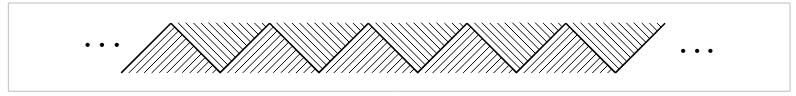
\includegraphics[scale=0.5]{Screenshot 2025-07-20 at 19-46-35 AT.dvi - AT.pdf.png}
\item[(c)] Let $Z$ be the zigzag subspace of $Y$ homeomorphic to $\mathbb{R}$ indicated by the heavier line. Show there is a deformation retraction in the weak sense of $Y$ onto $Z$, but no true deformation retraction.
\end{enumerate}
\end{exercise}
\begin{proof}
\begin{enumerate}
\item[(a)] We define a homotopy \[f_t:X\to X:(a,b) \mapsto (a,b(1-t)).\] $f_t$ fixes $[0,1]\times\{0\}$, $f_0=\text{id}_X$ and $f_1$ is a retraction from $X$ to $[0,1]\times\{0\}$, so $f_t$ is a deformation retraction. Hence $[0,1]\times\{0\}$ is a deformation retract of $X$. Any point in $[0,1]\times\{0\}$ is then clearly a deformation retract of $[0,1]\times\{0\}$, so  $X$ deformation retracts to any point in $[0,1]\times\{0\}$ by transitivity. Now suppose $X$ deformation retracts to some other point $x\in X$. We can then find a neighbourhood $U$ of $x$ of the form $B_\epsilon(x)\cap X$ for some $\epsilon > 0$, which does not contain $[0,1]\times\{0\}$. However, $U$ is not path-connected, so there does not exist a neighbourhood $V\subset U$ of $x$ such that the inclusion map $V\hookrightarrow U$ is nullhomotopic; a contradiction.
\item[(b)] Define a homotopy $f_t:Y\to Y$ where $f_t(y)$ sends $y$ a distance of $t$ to the right along $Y$. Then $f_0=\text{id}_Y$ and $f_1(Y)=Z$, where $Z$ is the zigzag subspace of $Y$. $Z$ is contractible, being homeomorphic to $\mathbb{R}$, and hence there exists a homotopy $h_t:Z\to Z$ from $\text{id}_Z$ to a constant function. We can then define a homotopy $F_t:Y\to Y$ of $\text{id}_Y$ to a constant map by\[F_t(y)=\begin{cases}
    f_{2t}(y)\text{ if }0\leq t\leq\frac{1}{2},
    \\h_{2t-1}\circ f_1(y)\text{ if }\frac{1}{2}< t\leq 1.
\end{cases}\]

Now suppose $Y$ deformation retracts onto a point $y$. We can then find a sufficiently small open neighbourhood $U$ of $y$ such that for every neighbourhood $V\subset U$ of $y$, $U$ is not path-connected, and hence the inclusion map $V\hookrightarrow U$ is not nullhomotopic; a contradiction. Hence $Y$ does not deformation retract onto a point $y$.
\item[(c)] Since $Z$ deformation retracts onto a point, if there were a deformation retract of $Y$ onto $Z$, then there would be a deformation retract of $Y$ onto a point. However, (b) showed that this is not the case, and hence $Y$ does not deformation retract onto $Z$. However, the homotopy $f_t$ defined in (b) is a weak deformation retract of $Y$ onto $Z$.
\end{enumerate}
\end{proof}

\begin{exercise}
Fill in the details in the following construction from
[Edwards 1999] of a compact space $Y\subset\mathbb{R}^3$ with the
same properties as the space $Y$ in Exercise $6$, that is, $Y$
is contractible but does not deformation retract to any
point. To begin, let $X$ be the union of an infinite sequence of cones on the Cantor set arranged end-to-end,
as in the figure. Next, form the one-point compactification of $X\times\mathbb{R}$. This embeds in $\mathbb{R}^3$ as a closed disk with curved ‘fins’ attached along circular arcs, and with the one-point compactification of $X$ as a cross-sectional slice.
The desired space $Y$ is then obtained from this subspace of $\mathbb{R}^3$ by wrapping one more
cone on the Cantor set around the boundary of the disk.

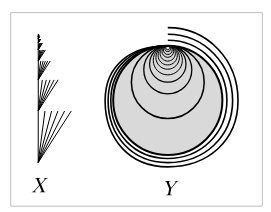
\includegraphics[scale=0.5]{Screenshot 2025-07-21 at 17-47-12 AT.dvi - AT.pdf.png}
\end{exercise}

\begin{exercise}
For $n>2$, construct an $n$-room analog of the house with two rooms.
\end{exercise}

\begin{exercise}
Show that a retract of a contractible space is contractible.
\end{exercise}
\begin{proof}
Let $X$ be a contractible space with $A$ a retract of $X$. Let $f_t:X\to X$ be a homotopy from $\text{id}_X$ to a constant map, and let $r:X\to A$ be a retraction of $X$ onto $A$. $r\circ {f_0}_{|A}=\text{id}_A$ and $r\circ {f_1}_{|A}$ is constant due to ${f_1}_{|A}$ being constant. Hence $\text{id}_A$ is homotopic to a constant map so $A$ is contractible.
\end{proof}

\begin{exercise}
Show that a space $X$ is contractible iff every map $f:X\to Y$, for arbitrary $Y$, is
nullhomotopic. Similarly, show $X$ is contractible iff every map $f:Y\to X$ is nullhomotopic.
\end{exercise}
\begin{proof}
$(\impliedby)$: Let $Y=X$ and $f=\text{id}_X$. Then $\text{id}_X$ is nullhomotopic so $X$ is contractible.

$(\implies)$: Let $g_t:X\to X$ be a homotopy from $\text{id}_X$ to a constant map. Then define a homotopy $h_t:X\to Y$ by $h_t(x)=f\circ g_t(x)$. This is a homotopy between $f$ and a constant map, so $f$ is nullhomotopic.

$(\impliedby)$: Again, let $Y=X$ and $f=\text{id}_X$.

$(\implies)$: $g_t\circ f$ is a homotopy from $f$ to a constant map so $f$ is nullhomotopic.
\end{proof}

\begin{exercise}
Show that $f:X\to Y$ is a homotopy equivalence if there exist maps $g,h:Y\to X$ such that $fg\simeq\mathbb{1}$ and $hf\simeq\mathbb{1}$. More generally, show that $f$ is a homotopy equivalence if $fg$ and $hf$ are homotopy equivalences.
\end{exercise}
\begin{proof}
Let $\phi=h\circ f\circ g:Y\to X$. Then\[f\circ\phi=f\circ(h\circ f\circ g)=f\circ(h\circ f)\circ g\simeq f\circ g\simeq\mathbb{1}\] and\[\phi\circ f=(h\circ f\circ g)\circ f=h\circ(f\circ g)\circ f\simeq h\circ f\simeq\mathbb{1}\] so $\phi$ is a homotopy inverse of $f$ so $f$ is a homotopy equivalence.

Let $g_1$ and $h_1$ be the homotopy inverses of $fg$ and $hf$ respectively. We then have that $f(gg_1)\simeq\mathbb{1}$ and $(h_1h)f\simeq\mathbb{1}$, and hence $f$ is a homotopy equivalence with homotopy inverse $h_1hfgg_1$.
\end{proof}

\begin{exercise}
Show that a homotopy equivalence $f:X\to Y$ induces a bijection between the set of path-components of $X$ and the set of path-components of $Y$, and that $f$ restricts to
a homotopy equivalence from each path-component of $X$ to the corresponding path-component of $Y$. Prove also the corresponding statements with components instead
of path-components. Deduce that if the components of a space $X$ coincide with its
path-components, then the same holds for any space $Y$ homotopy equivalent to $X$.
\end{exercise}
\begin{proof}
Let $\sim_X$ be the equivalence relation on $X$ given by $a\sim_X b$ if and only if $a$ and $b$ are in the same path-component. Similarly define the relation $\sim_Y$ on $Y$. Let $g:Y\to X$ be a homotopy inverse of $f$. We let $\phi_t$ and $\psi_t$ be homotopies from $\text{id}_Y$ to $f\circ g$ and from $\text{id}_X$ to $g\circ f$ respectively.


\textbf{We first show that $f$ induces a well-defined map on path components.}\\Let $x_0\sim_X x_1$. Let $\phi:I\to X$ be a path from $x_0$ to $x_1$. Then $f\circ\phi:I\to Y$ is a path from $f(x_0)$ to $f(x_1)$ so $f(x_0)\sim_Y f(x_1)$.

\textbf{We now show that $f$ induces a surjective map on path components.}\\Let $y\in Y$. Then $y=\phi_0(y)\sim_Y \phi_1(y)=f(g(y))$, and hence $y$ is in the same path component as a point in the image of $f$.

\textbf{We finally show that $f$ induces an injective map on path components.}\\ Suppose that $f(x_0)\sim_Yf(x_1)$. Then $g\circ f(x_0)\sim_X g\circ f(x_1)$ and hence $\psi_1(x_0)\sim_X\psi_1(x_1)$. We also have that $x_0=\psi_0(x_0)\sim_X\psi_1(x_0)$ and $x_1=\psi_0(x_1)\sim_X\psi_1(x_1)$, and so by transitivity\[x_0\sim_X\psi_1(x_0)\sim_X\psi_1(x_1)\sim_X x_1\implies x_0\sim_X x_1.\]Hence $f$ induces a bijection on path-components.\newline

Let $[x]_X$ be the path component of some point $x\in X$ and let $[f(x)]_Y$ be the path component in $Y$ of $f(x)$. $f$ then restricts to a map \[f_{|[x]_X}:[x]_X\to [f(x)]_Y.\] Furthermore, $g\circ f(x)\sim_X x$, and hence $g$ also restricts to a map \[g_{|[f(x)]_Y}:[f(x)]_Y\to[x]_X.\] We can then also restrict the homotopies $\phi_t$ and $\psi_t$ to \[\phi_{t|[f(x)]_Y}:[f(x)]_Y\to[f(x)]_Y\] and \[\psi_{t|[x]_X}:[x]_X\to[x]_X\] respectively, since $\forall x_0\in[x]_X$ we have $\psi_t(x_0)\sim_Xx_0\forall t$, and $\forall y_0\in[f(x)]_Y$ we have $\phi_t(y_0)\sim_Y y_0\forall t$. Hence $f_{|[x]_X}$ is a homotopy equivalence between $[x]_X$ and $[f(x)]_Y$.

Now let $\sim_X$ and $\sim_Y$ be the corresponding relations for connected components.

\textbf{We first show that $f$ induces a well-defined map on connected components.}
Let $x_0\sim_X x_1$. Let $Z$ be a connected subspace containing $x_0$ and $x_1$. The image of a connected space is connected, and hence $f(x_0)\sim_Y f(x_1)$, as both are contained in $f(Z)$.

\textbf{We next show that $f$ induces a surjective map on connected components.}
Let $y\in Y$. Let $[y]_Y$ be the connected component of $y$. As show earlier, $y$ is in the same path component as $f\circ g(y)$, and hence is in the same connected component as $f\circ g(y)$. Hence, $[y]_Y$ is in the image of the map on connected components induced by $f$.

\textbf{We finally show that $f$ induces an injective map on connected components.}
Let $f(x_0)\sim_Yf(x_1)$. Then $g\circ f(x_0)\sim_X g\circ f(x_1)$. We then have that $x_0$ is in the same path-component as $g\circ f(x_0)$ and $x_1$ is in the same path-component as $g\circ f(x_1)$, and hence that $x_0$ is in the same connected component as $g\circ f(x_0)$ and $x_1$ is in the same connected component as $g\circ f(x_1)$. Hence by transitivity\[x_0\sim_X g\circ f(x_0)\sim_Xg\circ f(x_1)\sim_X x_1\implies x_0\sim_X x_1.\] Hence $f$ induces a bijection on connected components.

Let $[x]_X$ be the connected component of some point $x\in X$ and let $[f(x)]_Y$ be the connected component of $f(x)$ in $Y$. $f$ then restricts to a map\[f_{|[x]_X}:[x]_X\to [f(x)]_Y.\]Furthermore, $g\circ f(x)\sim_X x$, and hence $g$ also restricts to a map \[g_{|[f(x)]_Y}:[f(x)]_Y\to[x]_X.\]We can then also restrict the homotopies $\phi_t$ and $\psi_t$ to \[\phi_{t|[f(x)]_Y}:[f(x)]_Y\to[f(x)]_Y\] and \[\psi_{t|[x]_X}:[x]_X\to[x]_X\] respectively, since $\forall x_0\in[x]_X$ we have $\psi_t(x_0)\sim_Xx_0\forall t$, and $\forall y_0\in[f(x)]_Y$ we have $\phi_t(y_0)\sim_Y y_0\forall t$. Hence $f_{|[x]_X}$ is a homotopy equivalence between $[x]_X$ and $[f(x)]_Y$.

Finally, suppose that the connected components of a space $X$ coincide with its path-components, and let $Y$ be homotopy equivalent to $X$. Let $f:X\to Y$ be a homotopy equivalence. Let \[f_\#:\{\text{Path/connected components of } X\}\to\{\text{Path components of } Y\}\] and \[f_*:\{\text{Path/connected components of } X\}\to\{\text{Connected components of } Y\}\] be the maps induced by $f$. We then have a bijection between path-components of $Y$ and connected components of $Y$ given by $f_*\circ f_\#^{-1}$. Furthermore, given any path-component $A\subseteq Y$, $f_*\circ f_\#^{-1}(A)$ is the connected component containing $A$. Hence there must be at most one path-component per connected component, since otherwise multiple path-components would be mapped to the same connected component by $f_*\circ f_\#^{-1}$, and it would cease to be injective. Hence the connected components of $Y$ coincide with its path-components.
\end{proof}

\begin{exercise}
Show that any two deformation retractions $r_t^0$ and $r_t^1$ of a space $X$ onto a subspace $A$ can be joined by a continuous family of deformation retractions $r_t^s$, $0\leq s\leq 1$, of $X$ onto $A$, where continuity means that the map $X\times I\times I\to X$ sending $(x,s,t)$ to $r_t^s(x)$ is continuous.
\end{exercise}
\begin{proof}
We know what $r_t^s$ is on $X\times\{0,1\}\times I\cup A\times I\times I\cup X\times I\times\{0\}$.

\noindent Define $r_t^s$ by\[r_t^s(x)=\begin{cases}
    r_t^0\circ r_{2ts}^1(x)\text{ if } 0\leq s <\frac{1}{2},\\r_{2t(1-s)}^0\circ r_t^1(x)\text{ if }\frac{1}{2}\leq s\leq 1.
\end{cases}\] If $s=0$, then $r_t^0=r_t^0\circ r_0^1=r_t^0$.

\noindent If $s=1$, then $r_t^1=r_0^0\circ r_t^1=r_t^1$.

\noindent If $a\in A$, then $r_t^s(a)=a\forall s,t$.

\noindent If $t=0$, then $r_0^s=\text{id}_X\forall s$.

\noindent If $t=1$, then $r_1^0(x)\in A\forall x$ and $r_1^1(x)\in A\forall x$, and hence $r_1^s(x)\in A\forall x$.
\end{proof}

\begin{exercise}
Given positive integers $v$, $e$ and $f$ satisfying $v-e+f=2$, construct a cell structure on $S^2$ having $v$ $0$-cells, $e$ $1$-cells, and $f$ $2$-cells.
\end{exercise}
\begin{proof}
For $(v,e,f)=(2+m,m+n+1,n+1)$ with $m>0,n>1$, we can use the following construction: Begin with $0$-cells $e_1^0,...,e_{2+m}^0$. Then attach $n-2$ loops $e_1^1,...,e_{n-2}^1$ to $e_1^0$, and add two $1$-cells $e_{n-1}^1$ and $e_n^1$, each with one endpoint attached to $e_1^0$ and the other endpoint attached to $e_{2+m}^0$. Then add $1$-cells $e_{n+1}^1,...,e_{n+1+m}^1$, where $e_{n+i}^1$ is attached to $e_i^0$ and $e_{i+1}^0$. Then add $2$-cells $e_1^2,...,e_{n+1}^2$, where the first $n-2$ are attached to the $n-2$ loops, the next two are attached to $e_1^0\cup...\cup e_{2+m}^0\cup e_{n-1}^1\cup e_{n+1}^1\cup...e_{n+1+m}^1$ and $e_1^0\cup...\cup e_{2+m}^0\cup e_n^1\cup e_{n+1}^1\cup...e_{n+1+m}^1$ respectively. Finally, attach the last $2$-cell to $e_1^0\cup e_2^0\cup e_1^1\cup...\cup e_n^1$.

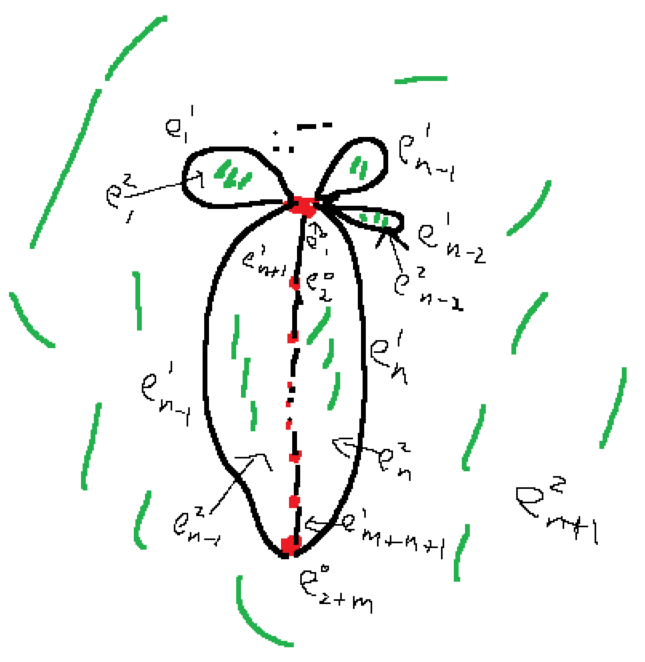
\includegraphics[scale=0.5]{Screenshot (1340).png}

If $v=2$, then $e=f$. First suppose $e>1$. We can then form $S^2$ by starting with $e_1^0$ and $e_2^0$, and then attaching $e-2$ loops to $e_1^0$ and two $1$-cells each connecting the two $0$-cells, and finally attaching $e$ $2$-cells.

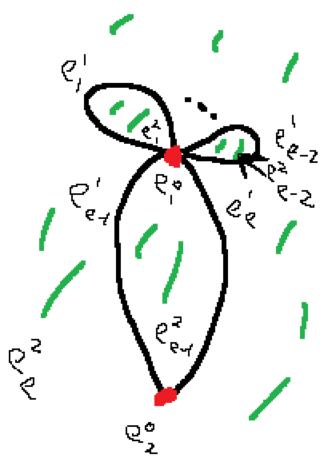
\includegraphics[scale=0.5]{Screenshot (1341).png}

The case $(v,e,f)=(2,1,1)$ is then just the standard construction of starting with two points, attaching two lines joining them to form a circle, filling in the centre of the circle, and then identifying the two lines.

Now consider the case $(v,e,f)=(2+m,m+2,2)$. That is, the case where $n=1$. The following diagram works:

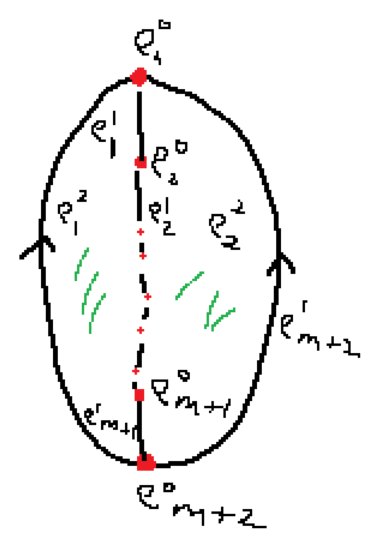
\includegraphics[scale=0.5]{Screenshot (1342).png}

For the case $(v,e,f)=(2+m,m+1,1)$, which corresponds to $n=0$, the following diagram works:

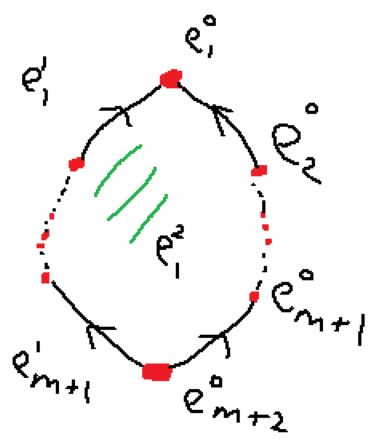
\includegraphics[scale=0.5]{Screenshot (1343).png}

For the case $(v,e,f)=(1,x,x+1)$, the following diagram works:

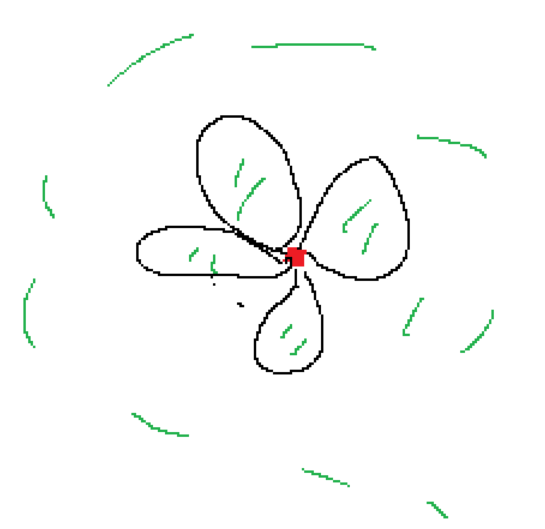
\includegraphics[scale=0.5]{Screenshot (1344).png}
\end{proof}

\begin{exercise}
Enumerate all the subcomplexes of $S^\infty$, with the cell structure on $S^\infty$ that has $S^n$ as its $n$-skeleton.
\end{exercise}
\begin{proof}
$X^n=S^n$ is a subcomplex of $S^\infty$ for every $n$. Also, for each $X^n=S^n$, $X^n\cup e_{1}^{n+1}$ and $X^n\cup e_{2}^{n+1}$ are subcomplexes. It is not possible to have a subcomplex formed by a proper subset of $X^n$ and some $\emptyset\neq\phi\subseteq X^{n+i}\setminus X^n$ for some $i\geq 1$, since $\phi$ attaches to the whole of $X^n$, and hence the subcomplex, being closed, would contain $X^n$; a contradiction. Hence, if a subcomplex contains an $i$-cell for $i>0$, it must also contain $X^{i-1}$. Hence the only possible subcomplexes are:
\[\emptyset, S^\infty, e_1^0,e_2^0, S^{i-1}\cup e_1^i,S^{i-1}\cup e_2^i \text{ for } i>0,\text{ and } S^n\text{ for }n\geq 0.\]
\end{proof}

\begin{exercise}
Show that $S^\infty$ is contractible.
\end{exercise}
\begin{proof}
For $k>0$, each $k$-skeleton $X^k\subseteq S^\infty$ is $S^{k-1}\cup e_1^k\cup e_2^k$, where $S^{k-1}\cup e_1^k$ and $S^{k-1}\cup e_2^k$ are both the disk $D^k$. Furthermore, for $k>1$, each $S^{k-1}\cup e_i^k$ can be deformation retracted into either $X^{k-2}\cup e_1^{k-1}$ or $X^{k-2}\cup e_2^{k-1}$. We can then repeat this recursively until we reach $X^0\cup e_i^{1}$, which we can then deformation retract to a single point in $X^0$. For $k>1$, let \[F_k:S^{k-1}\cup e_1^k\times I\to S^{k-1}\cup e_1^k\] be a deformation retraction of $S^{k-1}\cup e_1^k$ onto $X^{k-2}\cup e_1^{k-1}$, and for $k=1$, let \[F_1:X^0\cup e_1^1\times I\to X^0\cup e_1^1\] be a deformation retraction of $X^0\cup e_1^1$ onto $e_1^0$. Then, given an $x\in S^\infty$, let $n$ be the smallest positive integer such that $x\in X^{n-1}\cup e_1^n$. We then define a homotopy $h_t$ between $\text{id}_{S^\infty}$ and a constant map by\[h_t(x)=\begin{cases}
    x&\text{ if }0\leq t<\frac{1}{2^{n+1}},\\F_n(x,2^n(t-\frac{1}{2^{n+1}}))&\text{ if }\frac{1}{2^{n+1}}\leq t<\frac{1}{2^n},\\F_{n-1}(F_n(x,1),2^{n-1}(t-\frac{1}{2^{n}}))&\text{ if }\frac{1}{2^n}\leq t<\frac{1}{2^{n-1}},\\\vdots\\F_1(F_2(...F_n(x,1)...,1),2(t-\frac{1}{2}))&\text{ if }\frac{1}{2}\leq t\leq 1.
\end{cases}\]Since CW complexes have the weak topology with respect to their skeleta, a map is continuous if and only if its restriction to each skeleton is continuous. This is clearly the case for $h_t$, and hence $h_t$ is continuous.
\end{proof}

\begin{exercise}
\begin{enumerate}
\item[(a)] Show that the mapping cylinder of every map $f:S^1\to S^1$ is a CW complex.
\item[(b)] Construct a 2-dimensional CW complex that contains both an annulus $S^1\times I$ and a M\"obius band as deformation retracts.
\end{enumerate}
\end{exercise}
\begin{proof}
\begin{enumerate}
\item[(a)]
Observe the following diagram:


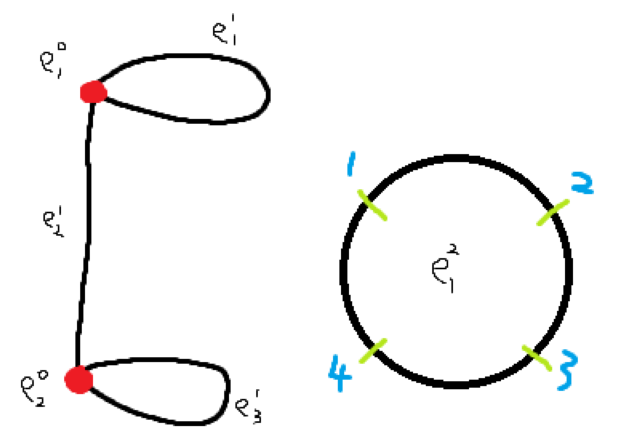
\includegraphics[scale=0.5]{Screenshot (1346).png}

We begin with a $1$-skeleton consisting of $e_1^0,e_2^0,e_1^1,e_2^1,e_3^1$. We then introduce a $2$-cell $e_1^2$. Let $\phi:S^1\to X^1$ be the attaching map of $e_1^2$. We define $\phi$ as follows: Identify the arc from $1$ to $2$ with $e_1^0\cup e_1^1$. Then identify the arc from $2$ to $3$ with $e_1^0\cup e_2^1\cup e_2^0$. Then identify the arc from $1$ to $4$ with $e_1^0\cup e_2^1\cup e_2^0$. Finally, let $A$ be the arc from $3$ to $4$. We then have homeomorphisms $g:A/3\sim 4\to S^1$ and $h:S^1\to e_3^1\cup e_2^0$ such that $h\circ f\circ g(3)=e_2^0$, and hence we can attach $A$ to $e_3^1$ under the identification $x\sim h\circ f\circ g(x)\forall x\in A$. This then gives a cell complex that is homeomorphic to $M_f$.
\item[(b)] We can form a CW complex out of gluing $S^1\times I$ to the midcircle of the M\"obius band, as in the diagram below:


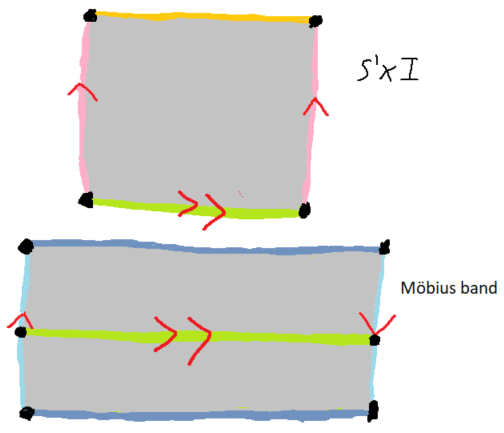
\includegraphics[scale=0.5]{Screenshot (1366).png}\newline We can then deformation retract $S^1\times I$ onto the midcircle of the M\"obius band, and we can deformation retract the M\"obius band onto $S^1\times I$ by deformation retracting it onto its midcircle, which is identified with $S^1\times\{0\}$.
\end{enumerate}
\end{proof}

\begin{exercise}
Show that $S^1*S^1=S^3$, and more generally $S^m*S^n=S^{m+n+1}$.
\end{exercise}
\begin{proof}
We can represent $S^1$ simply as $\{\theta:0\leq\theta<2\pi\}$, and hence $S^1\times S^1\times I\cong \{(\theta_0,\theta_1,r):0\leq\theta_0,\theta_1<2\pi,0\leq r\leq 1\}$. Then, applying the identifications gives\[S^1*S^1\cong\{(\theta_0,\theta_1,r):0\leq\theta_0,\theta_1<2\pi,0\leq r\leq 1\}/\sim,\]where\[(\theta_0,\theta_1,0)\sim(\theta_0,\theta_1',0)\forall \theta_0,\theta_1,\theta_1'\text{ and }(\theta_0,\theta_1,1)\sim(\theta_0',\theta_1,1)\forall \theta_0,\theta_0',\theta_1.\]

Now, $S^3$ is the set of pairs of complex numbers $(z_0,z_1)$ such that the squares of their norms sum to $1$. Representing them in polar coordinates then gives $z_0=r_0 e^{i\theta_0}$ and $z_1=r_1e^{i\theta_1}$, where $r_0^1+r_1^2=1$, $0\leq r_0,r_1\leq 1$ and $0\leq\theta_0,\theta_1<2\pi$. $r_1$ determines $r_0=\sqrt{1-r_1^2}$, so $(z_0,z_1)$ can be associated with a real triple $(\theta_0,\theta_1,r_1)$. However, in order to create a bijection, we need to make the following identifications:\[(\theta_0,\theta_1,0)\sim(\theta_0,\theta_1',0)\forall \theta_0,\theta_1,\theta_1'\] and \[(\theta_0,\theta_1,1)\sim(\theta_0',\theta_1,1)\forall\theta_0,\theta_0',\theta_1.\] These are exactly the identifications which give $S^1*S^1$, and hence $S^1*S^1=S^3$.
\newline

For the general case:

\noindent Recall that $SS^n=S^{n+1}$, and hence note that $S^n*S^0=SS^n=S^{n+1}$, which implies that \[S^n=\overset{n+1\text{ times}}{S^0*...*S^0}.\] Thus \[S^m*S^n=(\overset{n+1\text{ times}}{S^0*...*S^0})*(\overset{m+1\text{ times}}{S^0*...*S^0})=\overset{n+1+m+1\text{ times}}{S^0*...*S^0}=S^{m+n+1}.\]
\end{proof}

\begin{exercise}
Show that the space obtained from $S^2$ by attaching $n$ $2$-cells along any collection of $n$ circles in $S^2$ is homotopy equivalent to the wedge sum of $n+1$ $2$-spheres.
\end{exercise}
\begin{proof}
Let $A$ be the space obtained from $S^2$ by attaching $n$ $2$-cells. We can give $A$ a cell-complex structure as follows: We start with $n$ discs $A_1,...,A_n$, and we then draw lines between them such that the outer circles form part of a perimeter, and every region within the perimeter includes at most one circle $A_i$. Then attach $2$-cells to fill in the area within the perimeter, and another $2$-cell to the whole perimeter. This is shown in the following diagram: 

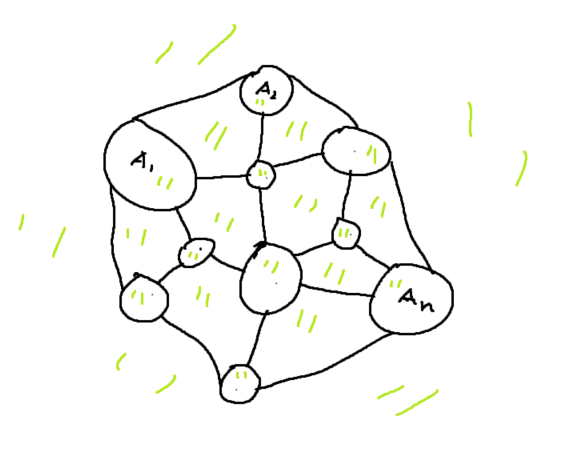
\includegraphics[scale=0.5]{Screenshot (1351).png}


We can then attach $n$ $2$-cells to the boundaries of the regions $A_1,...,A_n$ to get a space homeomorphic to $A$. Each $A_i$ is a contractible subcomplex, and hence we can collapse each $A_i$ to a point to obtain a space $B$ homotopy-equivalent to $A$, which consists of a sphere $S^2$ with $n$ other spheres attached to it at different points. We can then model $B$ as a cell-complex by starting with the points where the spheres are attached to the first sphere as $0$-cells, then adding $1$-cells to form a connected graph, then attaching $2$-cells to form a sphere, and then attaching $n$ more $2$-cells to each $0$-cell, as shown in the following diagram:

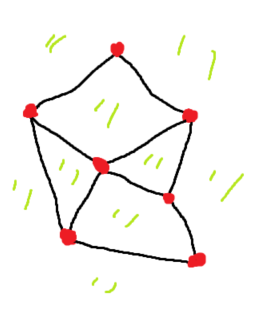
\includegraphics[scale=0.5]{Screenshot (1352).png} 

We can then repeatedly collapse each pair of vertices connected by an edge to a point, so as to end up with $\bigvee_{i=1}^{n+1}S^2$, which will be homotopy equivalent to $A$.
\end{proof}

\begin{exercise}
Show that the subspace $X\subset\mathbb{R}^3$ formed by a Klein bottle intersecting itself in a circle, as shown in the figure, is homotopy equivalent to $S^1\vee S^1\vee S^2$.

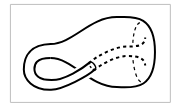
\includegraphics[scale=0.5]{Screenshot 2025-08-06 at 01-25-18 AT.dvi - AT.pdf.png}
\end{exercise}
\begin{proof}
First, we can collapse the disc whose boundary is the circle of intersection to a point, to obtain the $2$-sphere with $3$ distinct points identified. This is then homotopy equivalent to the diagram below, since we can collapse both segments $a$ and $b$ to obtain a sphere with three distinct points identified.

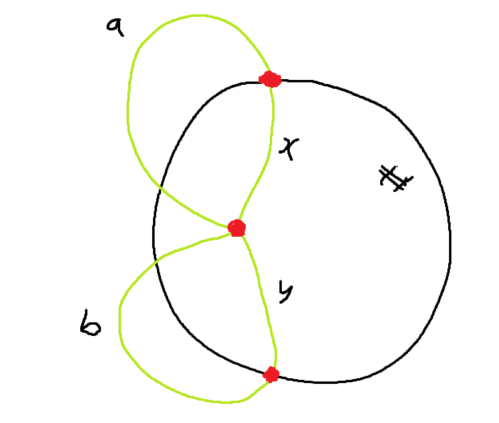
\includegraphics[scale=0.5]{Screenshot (1355).png}

\noindent However, we can also collapse the segments $x$ and $y$ instead, which then gives $S^1\vee S^1\vee S^2$, as required.
\end{proof}

\begin{exercise}
If $X$ is a connected Hausdorff space that is a union of a finite number of $2$-spheres, any two of which intersect in at most one point, show that $X$ is homotopy equivalent to a wedge sum of $S^1$'s and $S^2$'s.
\end{exercise}
\begin{proof}
Firstly, we can represent the spheres as a simple connected graph, where each vertex represents a sphere, and two vertices being connected by an edge represents two spheres intersecting at a point. Let $T$ be a spanning tree of the graph. We can construct a CW complex of $X$ as follows: For each sphere $X_i$, let $A_i$ be the set of points of intersection of $X_i$ with other spheres which are connected to $X_i$ by an edge in $T$, and let $B_i$ be the set of points of intersection of $X_i$ with other spheres which are connected to $X_i$ by an edge not in $T$. Let $C_i$ be a copy of $B_i$, so that $\left|\bigcup_{i=1}^nC_i\right|=|\bigsqcup_{i=1}^nB_i|$. We then form a $0$-skeleton consisting of $0$-cells which correspond to the points in $A_1\cup...\cup A_n$ and $C_1\cup...\cup C_n$. For each $i$, we connect all the points in $A_i\cup C_i$ by $1$-cells, so as to form a simple acyclic graph, which we shall denote as $G_i$. We then connect each pair of points in $C_i\cup C_j$ which correspond to a single point in $B_i$ with a $1$-cell. Finally, we attach a $2$-cell to each $G_i$, which then gives a space that is homotopy equivalent to $X$; for we can collapse the $1$-cells connecting the points in $C_1\cup...\cup C_n$ to obtain all the intersections. This is illustrated in the following diagram, where the black circles represent $2$-spheres, the green dots represent points in $C_1\cup...\cup C_n$, the red dots represent points in $A_1\cup...\cup A_n$, the purple lines represent $G_i$'s, and the blue line represents a $1$ cell connecting to points in $C_1\cup...\cup C_n$.

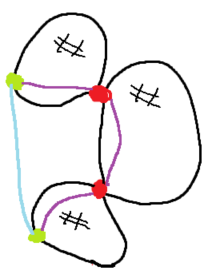
\includegraphics[scale=0.5]{Screenshot (1361).png}

If we instead collapse each $G_i$ to a point, we then obtain a wedge sum of $n$ $2$-spheres, along with the loops corresponding to the $1$-cells connecting the points in $C_1\cup...\cup C_n$, which are now all the same point.
\end{proof}

\begin{exercise}
Let $X$ be a finite graph lying in a half-plane $P\subseteq \mathbb{R}^3$ and intersecting the edge of $P$ in a subset of the vertices of $X$. Describe the homotopy type of the 'surface of revolution' obtained by rotating $X$ about the edge line of $P$.
\end{exercise}
\begin{proof}
First, assume that $X$ is connected. Without loss of generality, we can assume that none of the edges of $X$ intersect, for if they do, then we can simply add a vertex at the point of intersection. We first consider three subgraphs of $X$:
\begin{enumerate}
\item The first, which we shall denote as $T$, is a spanning forest of the collection of vertices of $X$ which do not lie in $\partial P$.
\item The second, which we shall denote as $A$, consists of all the edges of $X$ which are not part of $T$, and which do not have an endpoint on $\partial P$, along with their endpoints.
\item The third, which we shall denote as $B$, consists of all vertices on $\partial P$, all vertices of $X$ which are connected to a vertex on $\partial P$ by an edge, and all edges which have an endpoint in $\partial P$.
\end{enumerate} Let $T_1,...,T_n$ be the spanning trees which comprise $T$. Let $V_{T_i}$ be the subcomplex of $T_i$ formed by all the vertices of $T_i$, let $v_i$ be a vertex in $T_i$ that is connected to a vertex in $\partial P$ by an edge, let $V_A$ be all the vertices of $A$, and let $V_B:=\{w_1,...,w_m\}$ be all vertices in $B$ which do not lie on $\partial P$. If we define a map $f:V_A\sqcup V_B\to T$ which maps the vertices of $V_A\sqcup V_B$ to their appropriate vertices in $T$, we then have that $X\cong T\sqcup_f(A\sqcup B)$. We can then define a map $g:V_A\sqcup V_B\to T$ which maps every vertex of $V_A\sqcup V_B$ to some $v_i$. Clearly $f\simeq g$. Let \[F:(V_A\sqcup V_B)\times I\to T\] be a homotopy from $f$ to $g$. We can then obtain a homotopy \[G:(V_A\sqcup V_B)\times S^1\times I\to T\times S^1:(v,\omega,t)\mapsto(F(v,t),\omega).\] Continuity of $G$ follows from the universal property of the product topology, for \[\pi_T\circ G:(V_A\sqcup V_B)\times S^1\times I\to T:(v,\omega,t)\mapsto F(v,t)\] and \[\pi_{S^1}\circ G:(V_A\sqcup V_B)\times S^1\times I\to S^1:(v,\omega,t)\mapsto \omega\] are both continuous. Define \[\alpha:(V_A\sqcup V_B)\times S^1\to T\times S^1:(v,\omega)\mapsto G(v,\omega,0)\] and \[\beta:(V_A\sqcup V_B)\times S^1\to T\times S^1:(v,\omega)\mapsto G(v,\omega,1).\] Let $Y$ be the resulting space after rotating $X$ about $\partial P$, which is homeomorphic to \[(X\times S^1)/\sim,\] where $\sim$ is given by $(v,\omega)\sim(v,\omega')\forall \omega, v\in X^0\cap \partial P$. Then if we define a relation $\sim_B$ on $(A\sqcup B)\times S^1$ given by $(v,\omega)\sim_B(v,\omega')\forall v\in \partial P,\omega\in S^1$, we have \begin{align*}Y&\cong (T\times S^1)\sqcup_\alpha(((A\sqcup B)\times S^1)/\sim_B)\\&\simeq(T\times S^1)\sqcup_\beta(((A\sqcup B)\times S^1)/\sim_B)\\&\simeq(\{v_1,...,v_n\}\times S^1)\sqcup_{r\circ\beta}(((A\sqcup B)\times S^1)/\sim_B),\end{align*} where the last homotopy equivalence was obtained by deformation retracting $T\times S^1$ to $\{v_1,...,v_n\}\times S^1$, and letting $r:T\times S^1\to \{v_1,...,v_n\}\times S^1$ be a retraction. Let $q$ be the number of edges in $A$. Then the joining of $A$ to $\{v_1,...,v_n\}\times S^1$ amounts to attaching $q$ $2$-tori onto $\{v_1,...,v_n\}\times S^1$ around a longitude. Finally, for each $i$, we choose a subspace $B_i$ which consists of $v_i\times S^1$, a vertex in $\partial P$ which is connected to $v_i$ by a disk, and the connecting disk itself. Each $B_i$ is a contractible subcomplex, and hence we can collapse it to a point. Then all the disks formed from the edges of $B$ will become $2$-spheres or horn tori, and the tori formed from the edges of $A$ will also become horn tori. Moreover, each horn torus, being formed by a loop with a basepoint on $\partial P$ being rotated about $\partial P$, is homeomorphic to semicircle (with the line of the semicircle lying on $\partial P$) being rotated around $\partial P$ and then having the line collapsed to a point. That is in turn homotopy equivalent to $S^2\vee S^1$, for we can move one of the attaching points of the line to the other point. This is illustrated in the diagram below:

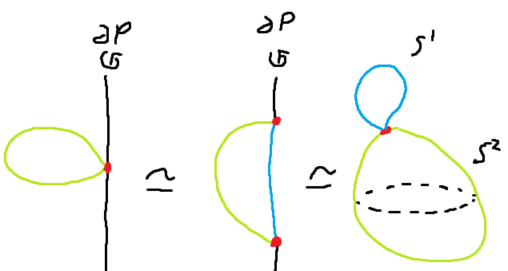
\includegraphics[scale=0.5]{Screenshot (1377).png}

\noindent We finish by repeating the following procedure: We choose a pair of vertices on $\partial P$ which are the endpoints of a sphere, and we choose one such sphere and collapse a contractible arc on the sphere connecting those two vertices. This will maintain the homotopy type of the sphere, while identifying two points on the other such spheres, which then gives them the homotopy types of $S^2\vee S^1$. We repeat this until every vertex is identified with every other, which is possible, due to $X$ being connected. The end result is a wedge sum of circles and spheres.
\end{proof}

\begin{exercise}
Show that a CW complex is contractible if it is the union of two contractible subcomplexes whose intersection is also contractible.
\end{exercise}
\begin{proof}
Let $X$ be a CW complex which is a union of contractible subcomplexes $A$ and $B$, where $A\cap B$ is also contractible. Then $X\simeq X/A\cong B/(A\cap B)\simeq B\simeq\{\text{pt}\}$.
\end{proof}

\begin{exercise}
Let $X$ and $Y$ be CW complexes with $0$-cells $x_0$ and $y_0$. Show that the quotient spaces $X*Y/(X*\{y_0\}\cup\{x_0\}*Y)$ and $S(X\wedge Y)/S(\{x_0\}\wedge\{y_0\})$ are homeomorphic, and deduce that $X*Y\simeq S(X\wedge Y)$.
\end{exercise}
\begin{proof}
\begin{align*}\{x_0\}\wedge\{y_0\}&=(\{x_0\}\times\{y_0\})/(\{x_0\}\times\{y_0\}\cup\{x_0\}\times\{y_0\})\\&=\{(x_0,y_0)\}/\{(x_0,y_0)\}\\&=\{(x_0,y_0)\}.\end{align*}and hence\[S(\{x_0\}\wedge\{y_0\})=S\{(x_0,y_0)\}=\{(x_0,y_0)\}\times I.\]
Furthermore,
\begin{align*}
S(X\wedge Y)&=S(X\times Y/(\{x_0\}\times Y\cup X\times\{y_0\}))\\&=X\times Y\times I/\sim
\end{align*}where \begin{align*}(x,y,0)&\sim(x',y',0)&\forall x,y,x',y',\\ (x,y,1)&\sim(x',y',1)&\forall x,y,x',y',\\(x_0,y,t)&\sim(x_0,y_0,t)&\forall y,t,\\ (x,y_0,t)&\sim(x_0,y_0,t)&\forall x,t.\end{align*} Hence \[S(X\wedge Y)/S(\{x_0\}\wedge\{y_0\})=X\times Y\times I/\sim\]where\begin{align*}(x,y,0)&\sim(x',y',0)&\forall x,y,x',y',\\ (x,y,1)&\sim(x',y',1)&\forall x,y,x',y',\\(x_0,y,t)&\sim(x_0,y_0,0)&\forall y,t,\\ (x,y_0,t)&\sim(x_0,y_0,0)&\forall x,t.\end{align*} which simplifies to \begin{align*}(x,y,0)&\sim(x_0,y_0,0)&\forall x,y,\\ (x,y,1)&\sim(x_0,y_0,0)&\forall x,y,\\(x_0,y,t)&\sim(x_0,y_0,0)&\forall y,t,\\ (x,y_0,t)&\sim(x_0,y_0,0)&\forall x,t.\end{align*}Next,
\[X*Y=X\times Y\times I/\sim\] where \begin{align*}
(x,y,0)&\sim(x,y',0)&\forall x,y,y'\\(x,y,1)&\sim(x',y,1)&\forall x,x',y
\end{align*}Furthermore, \[X*\{y_0\}\cup \{x_0\}*Y=(X\times\{y_0\}\times I\cup \{x_0\}\times Y\times I)/\sim\]where\begin{align*}
(x_0,y,0)&\sim(x_0,y',0)&\forall y,y'\\(x,y_0,1)&\sim(x',y_0,1)&\forall x,x'
\end{align*}and hence\[X*Y/(X*\{y_0\}\cup\{x_0\}*Y)=X\times Y\times I/\sim\]where\begin{align*}
(x,y,0)&\sim(x,y',0)&\forall x,y,y'\\(x,y,1)&\sim(x',y,1)&\forall x,x',y\\(x,y_0,t)&\sim(x_0,y_0,0)&\forall x_,t\\(x_0,y,t)&\sim(x_0,y_0,0)&\forall y,t\\(x_0,y,0)&\sim(x_0,y',0)&\forall y,y'\\(x,y_0,1)&\sim(x',y_0,1)&\forall x,x'
\end{align*} which simplifies to \begin{align*}
(x,y,0)&\sim(x,y',0)&\forall x,y,y'\\(x,y,1)&\sim(x',y,1)&\forall x,x',y\\(x,y_0,t)&\sim(x_0,y_0,0)&\forall x_,t\\(x_0,y,t)&\sim(x_0,y_0,0)&\forall y,t
\end{align*}Furthermore,\[(x,y,0)\sim(x,y_0,0)\sim(x_0,y_0,0)\forall x,y,\] and \[(x,y,1)\sim(x_0,y,1)\sim(x_0,y_0,0)\forall x,y.\] So the final simplification is\begin{align*}
(x,y,0)&\sim(x_0,y_0,0)&\forall x,y\\(x,y,1)&\sim(x_0,y_0,1)&\forall x,y\\(x,y_0,t)&\sim(x_0,y_0,0)&\forall x_,t\\(x_0,y,t)&\sim(x_0,y_0,0)&\forall y,t
\end{align*}These identifications are identical to the identifications which yield $S(X\wedge Y)/S(\{x_0\}\wedge\{y_0\})$, and hence \[X*Y/(X*\{y_0\}\cup\{x_0\}*Y)\cong S(X\wedge Y)/S(\{x_0\}\wedge\{y_0\}).\]
Finally, both $(X*\{y_0\}\cup\{x_0\}*Y)$ and $S(\{x_0\}\wedge\{y_0\})$ are contractible subcomplexes, and hence\[X*Y\simeq X*Y/(X*\{y_0\}\cup\{x_0\}*Y)\cong S(X\wedge Y)/S(\{x_0\}\wedge\{y_0\})\simeq S(X\wedge Y).\]
\end{proof}

\begin{exercise}
If $X$ is a CW complex with components $X_\alpha$, show that the suspension $SX$ is homotopy equivalent to $Y\bigvee_\alpha SX_\alpha$ for some graph $Y$. In the case that $X$ is a finite graph, show that $SX$ is homotopy equivalent to a wedge sum of circles and $2$-spheres.
\end{exercise}
\begin{proof}
$SX\cong(\coprod_\alpha X_\alpha\times I)/\sim$, where\begin{align*}
\forall\alpha:(x,0)&\sim(x',0)&\forall x,x'\in X_\alpha\\\forall\alpha:(x,1)&\sim(x',1)&\forall x,x'\in X_\alpha
\end{align*} and hence if we select an $x_\alpha\in X_\alpha\forall\alpha$, we have $SX\cong(\coprod_\alpha SX_\alpha)/\sim$ where\begin{align*}
[(x_\alpha,0)]&\sim[(x_{\alpha'},0)]&\forall \alpha,\alpha'\\ [(x_\alpha,1)]&\sim[(x_{\alpha'},1)]&\forall \alpha,\alpha'
\end{align*} This can then be expressed as the quotient of a wedge sum with chosen points $[(x_\alpha,0)]$ as follows:\[\left.SX\cong\left(\bigvee_\alpha SX_\alpha\right)\middle/\sim\right.\] where\[[(x_\alpha,1)]\sim[(x_{\alpha'},1)]\forall \alpha,\alpha'.\]Now let $G$ be a connected acyclic graph with vertices $v_\alpha$. Call the set of vertices the subcomplex $A$. Then define $f:A\to \bigvee_\alpha SX_\alpha$ by $f(v_\alpha)=[(x_\alpha,1)]\forall\alpha$. It then follows that $SX\simeq\left(\bigvee_\alpha SX_\alpha\right)\sqcup_f G$, since we can collapse $G$ to identify every $[(x_\alpha,1)]$. Moreover, $f\simeq g$, where $g:A\to \bigvee_\alpha SX_\alpha$ maps every $v_\alpha$ to $[(x_\alpha,0)]$, and hence \[SX\simeq\left(\bigvee_\alpha SX_\alpha\right)\sqcup_f G\simeq\left(\bigvee_\alpha SX_\alpha\right)\sqcup_g G.\] $\left(\bigvee_\alpha SX_\alpha\right)\sqcup_g G$ is in turn homeomorphic to \[Y\bigvee_\alpha SX_\alpha,\] where $Y$ is a graph consisting of a single vertex and $l-1$ loops, where $l$ is the number of components of $X$.\newline

\noindent Now let $X$ be a finite graph. Let $T_\alpha$ be a spanning tree of $X_\alpha$, and let $n_\alpha$ be the number of edges in $X_\alpha$ that are not part of $T_\alpha$. $ST_\alpha$ is a contractible subcomplex, and every edge in $X_\alpha$ becomes a $2$-sphere in $SX_\alpha$. Hence, if $n_\alpha>0$, we have \[SX_\alpha\simeq S\left(\bigvee_{i=1}^{n_\alpha}S^1\right)\simeq\sum\left(\bigvee_{i=1}^{n_\alpha}S^1\right)=\bigvee_{i=1}^{n_\alpha}\sum S^1=\bigvee_{i=1}^{n_\alpha}S^2.\] Otherwise, if $n_\alpha=0$, then $SX_\alpha$ is simply contractible. If we define $\bigvee_{i=1}^0Q
$ to be a point for any space $Q$, we then have\[SX\simeq \bigvee_{i=1}^{l-1}S^1\bigvee_{i=1}^{\sum_\alpha n_\alpha}S^2,\] as required.
\end{proof}


\begin{exercise}
Use Corollary 0.20 to show that if $(X,A)$ has the homotopy extension property, then $X\times I$ deformation retracts to $X\times\{0\}\cup A\times I$. Deduce from this that Proposition 0.18 holds more generally for any pair $(X_1,A)$ satisfying the homotopy extension property.
\end{exercise}
\begin{proof}
Firstly, $(X\times I, X\times\{0\}\cup A\times I)$ also satisfies the homotopy extension property. Let \[\iota:X\times\{0\}\cup A\times I\to X\times I\] be the inclusion map. Define \[\phi:X\times I\to X\times\{0\}\cup A\times I:(x,s)\mapsto(x,0).\] Then \[\iota\circ \phi(x,s)=(x,0)\forall (x,s)\in X\times I.\] Define \[h_t:X\times I\to X\times I\] by \[h_t(x,s)=(x,ts).\] Then $h_0=\iota\circ\phi$ and $h_1=\text{id}_{X\times I}$, and hence \[\iota\circ\phi\simeq\text{id}_{X\times I}.\] Furthermore, \[\phi\circ\iota(x,s)=(x,0)\forall (x,s)\in X\times \{0\}\cup A\times I.\] Now define \[g_t:X\times\{0\}\cup A\times I\to X\times\{0\}\cup A\times I:(x,s)\mapsto(x,ts).\] Then $g_0=\phi\circ\iota$ and $g_1=\text{id}_{X\times\{0\}\cup A\times I}$, and hence \[\phi\circ\iota\simeq \text{id}_{X\times\{0\}\cup A\times I}.\] Corollary $0.20$ then implies that $X\times I$ deformation retracts to $X\times\{0\}\cup A\times I$.\newline


Now let $(X_1,A)$ be a pair satisfying the homotopy extension property, let $X_0$ be another topological space, and let $f,g:A\to X_0$ be homotopic. Let $F:A\times I\to X_0$ be a homotopy from $f$ to $g$. Consider the space $X_0\sqcup_F(X_1\times I)$. $X_1\times I$ deformation retracts onto $X_1\times\{0\}\cup A\times I$, and hence $X_0\sqcup_F(X_1\times I)$ deformation retracts onto $X_0\sqcup_F(X_1\times\{0\}\cup A\times I)$, which is in turn homeomorphic to $X_0\sqcup_fX_1$. Similarly, $X_1\times I$ deformation retracts onto $X_1\times\{1\}\cup A\times I$, and hence $X_0\sqcup_F(X_1\times I)$ deformation retracts onto $X_0\sqcup_gX_1$. Furthermore, these deformation retractions both fix $X_0$, and hence $X_0\sqcup_fX_1\simeq X_0\sqcup_gX_1\text{ rel }X_0$.
\end{proof}


\begin{exercise}
Given a pair $(X,A)$ and a homotopy equivalence $f:A\to B$, show that the natural map $X\to B\sqcup_fX$ is a homotopy equivalence if $(X,A)$ satisfies the homotopy extension property. An interesting case is when $f$ is a quotient map, hence the map $X\to B\sqcup_f X$ is the quotient map identifying each set $f^{-1}(b)$ to a point. When $B$ is a point this gives another proof of Proposition $0.17$.
\end{exercise}
\begin{proof}
By Corollary $0.21$, $A$ is a deformation retract of $M_f$, and hence $X$ is a deformation retract of $X\cup M_f$. By the previous exercise, $X\times\{0\}\cup A\times I$ is a deformation retract of $X\times I$, and hence $X\cup M_f$ is a deformation retract of $(X\times I)\sqcup B/\sim$, where $\sim$ is given by $(a,1)\sim f(a)\forall a\in A$. $(X\times I\sqcup B)/\sim$ in turn deformation retracts onto $(X\times\{1\}\sqcup B)/\sim$, which is homeomorphic to $B\sqcup_fX$.\[X\overset{\iota_1}{\longrightarrow} X\cup M_f\overset{\iota_2}{\longrightarrow} (X\times I\sqcup B)/\sim\overset{r}{\longrightarrow} B\sqcup_fX.\] $\iota_1:X\hookrightarrow X\cup M_f$ is a homotopy equivalence, $\iota_2:X\cup M_f\hookrightarrow (X\times I\sqcup B)/\sim$ is a homotopy equivalence, and the retraction $r:(X\times I\sqcup B)/\sim\to B\sqcup _fX$ given by $r([(x,s)])=[x]\forall (x,s)\in X\times I$ and $r([b])=[b]\forall b\in B$ is a homotopy equivalence. The composition of homotopy equivalences is a homotopy equivalence, and hence $r\circ \iota_2\circ\iota_1:X\to B\sqcup_fX$, which is precisely the natural map $X\to B\sqcup_fX$, is a homotopy equivalence.
\end{proof}

\begin{exercise}
Show that if $(X_1,A)$ satisfies the homotopy extension property, then so does every pair $(X_0\sqcup_fX_1,X_0)$ obtained by attaching $X_1$ to a space $X_0$ via a map $f:A\to X_0$.
\end{exercise}
\begin{proof}
Suppose we have a map $f_0:X_0\sqcup_fX_1\to Y$ and a homotopy $f_t:X_0\to Y$ of $f_0|X_0$. This in turn induces a homotopy on $A$ given by $f_t\circ f$. Since $(X_1,A)$ satisfies the HEP, it follows that $f_t\circ f:A\to Y$ can be extended to a homotopy $g_t:X_1\to Y$ with $g_0(x)=f_0([x])\forall x\in X_1$. We can thus extend $f_t$ to a homotopy $f_t:X_0\sqcup_fX_1\to Y$ given by \[f_t([x])=\begin{cases}
    g_t(x)&\text{if }x\in X_1,\\
    f_t(x)&\text{if }x\in X_0.
\end{cases}\]This is well-defined, for if $x\in A$, then $g_t(x)=f_t\circ f(x)=f_t([x])$. We now show that $f_t$ is continuous. First, define a homotopy \[F:(X_0\sqcup X_1)\times I\to Y:F(x,t)\mapsto f_t([x]).\] Let $\iota_0,\iota_1$ be the inclusion maps of $X_0$ and $X_1$ respectively into $X_0\sqcup X_1$. $\iota_0(X_0)\times I$ and $\iota_1(X_1)\times I$ are both closed in $(X_0\sqcup X_1)\times I$ as a consequence of the coproduct topology, \[\iota_0(X_0)\times I\cup \iota_1(X_1)\times I=(X_0\sqcup X_1)\times I,\] and $F$ is continuous when restricted to both $\iota_0(X_0)\times I$ and $\iota_1(X_1)\times I$, and hence $F$ is continuous on $(X_0\sqcup X_1)\times I$ by the Pasting lemma. Now let \[q:(X_0\sqcup X_1)\times I\to (X_0\sqcup_fX_1)\times I:(x,t)\mapsto([x],t)\] be the quotient map. $F$ then descends to a map \[G:(X_0\sqcup_fX_1)\times I\to Y:([x],t)\mapsto F(x,t),\] which is continuous by the universal property of the final topology, since $F=G\circ q$. Finally, \[G([x],t)=f_t([x])\forall[x]\in X_0\sqcup_fX_1,\] and hence $f_t$ is continuous, so a homotopy. Thus $(X_0\sqcup_fX_1,X_0)$ has the HEP. 
\newline Note - To justify that $q$ is actually a quotient map, we invoke the following result from "General Topology" by Engelking (theorem 3.3.17):\newline

\noindent Let $X$  be a locally compact space. Let $q:Y\to Z$ be a quotient map. Let the map \[f:X\times Y\to X\times Z\] be defined by $f(x,y)=(x,q(y))$ for each $(x,y)\in X\times Y$. Then the map $f$ is a quotient map from $X\times Y$ to $X\times Z$.

Indeed, $I$ is a compact Hausdorff space, and hence locally compact, so the result applies.
\end{proof}

\begin{exercise}
In case the CW complex $X$ is obtained from a subcomplex $A$ by attaching a single cell $e^n$, describe exactly what the extension of a homotopy $f_t:A\to Y$ to $X$ given by the proof of Proposition $0.16$ looks like. That is, for a point $x\in e^n$, describe the path $f_t(x)$ for the extended $f_t$.
\end{exercise}
\begin{proof}
Define $F:X\times I\to Y$ by $F(x,t)=f_t(x)$. The extension of $F:X\times\{0\}\cup A\times I\to Y$ is simply $F\circ R:X\times I\to Y$, where $R$ is the retraction of $X\times I$ to $X\times\{0\}\cup A\times I$ given in Proposition 0.16.

Let $r:D^n\times I\to D^n\times\{0\}\cup \partial D^n\times I$ be the retraction of $D^n\times I$ described in Proposition 0.16. 
We consider three different cases:
\begin{enumerate}
\item If $x$ is in the centre of $e^n$, then $r(x,t)=(x,0)\forall t\in I$. 
\item If $2-2\|x\|> 1$, then $r(x,t)$ simply moves $x$ radially outwards from the centre towards $\frac{x}{\|x\|}$ as $t$ increases, while keeping the $I$ component at $0$. In particular, if $p_x:I\to D^n:t\mapsto\frac{2x}{2-t}$ is the line $x$ travels on outwards from the centre as $t$ increases, then we have $r(x,t)=(p_x(t),0)$.
\item Otherwise,  $r(x,t)$ moves radially outwards from $(x,0)$ at $t=0$ to $\left(\frac{x}{\|x\|},0\right)$ at $t=2-2\|x\|$. For $t\geq2-2\|x\|$, we simply increase the value of the $I$ component. Explicitly, if we let $p_x:[0,2-2\|x\|]\to D^n:t\mapsto\frac{2x}{2-t}$ be the line from $x$ to $\frac{x}{\|x\|}$, then\[r(x,t)=\begin{cases}
    (p_x(t),0)&\text{if }t< 2-2\|x\|,\\
    \left(\frac{x}{\|x\|},2-\frac{2-t}{\|x\|}\right)&\text{if }t\geq2-2\|x\|.
\end{cases}\]
\end{enumerate}
We can now describe the path of $f_t(x)$. Let $\phi:\partial D^n\to A$ be the attaching map of $e^n$.
\begin{enumerate}
\item In the first situation, where $x$ is in the centre of $e^n$, then $f_t(x)=f_0(x)\forall t$.
\item In the second situation, where $2-2\|x\|> 1$, then $f_t(x)=f_0\left(\frac{2x}{2-t}\right)\forall t$.
\item In the final situation, where $2-2\|x\|\leq 1$, then\[f_t(x)=\begin{cases}
    f_0\left(\frac{2x}{2-t}\right)&\text{if }t<2-2\|x\|,\\
    f_{2-\frac{2-t}{\|x\|}}\circ\phi\left(\frac{x}{\|x\|}\right)&\text{if }t\geq 2-2\|x\|.
\end{cases}\]
\end{enumerate}
\end{proof}
\section{The Fundamental Group}
\subsection{Basic Constructions}
\end{document}
